\subsection{Caso d'uso UC7: Creazione di un progetto}
\begin{figure}[h] 
	\centering 
	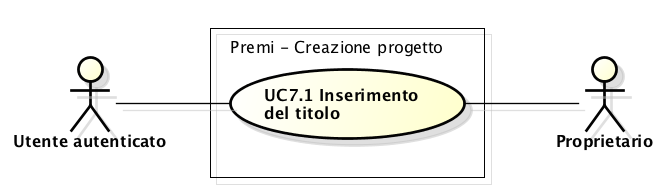
\includegraphics[scale=0.45] {img/UC7.png}
	\caption{UC7 - Creazione di un progetto} 
\end{figure}

\begin{itemize}
	\item \textbf{Attori:} Proprietario;
	\item \textbf{Scopo e descrizione:} L'utente vuole creare un nuovo progetto. Ha la possibilità di decidere il titolo del progetto e il \gls{template} con cui crearlo. Successivamente passerà alla fase di modifica.
	\item \textbf{Precondizione:} L'utente deve aver eseguito l'accesso al sistema;
	\item \textbf{Flusso principale degli eventi:}
	\begin{enumerate}
		\item L'utente sceglie il titolo [UC7.1].
	\end{enumerate}
	\item \textbf{Postcondizione:} Il sistema registra le scelte dell'utente ed entra nella modalità di modifica del progetto.
\end{itemize}


\subsection{Caso d'uso UC7.1: Scegliere il titolo}
\begin{itemize}
	\item \textbf{Attori:} Proprietario;
	\item \textbf{Scopo e descrizione:} L'utente sceglie il titolo da dare al progetto;
	\item \textbf{Precondizione:} L'utente ha deciso di creare un nuovo progetto;
	\item \textbf{Postcondizione:} Il sistema registra il titolo inserito dall'utente.
\end{itemize}